\documentclass[twoside]{book}

% Packages required by doxygen
\usepackage{fixltx2e}
\usepackage{calc}
\usepackage{doxygen}
\usepackage[export]{adjustbox} % also loads graphicx
\usepackage{graphicx}
\usepackage[utf8]{inputenc}
\usepackage{makeidx}
\usepackage{multicol}
\usepackage{multirow}
\PassOptionsToPackage{warn}{textcomp}
\usepackage{textcomp}
\usepackage[nointegrals]{wasysym}
\usepackage[table]{xcolor}

% Font selection
\usepackage[T1]{fontenc}
\usepackage[scaled=.90]{helvet}
\usepackage{courier}
\usepackage{amssymb}
\usepackage{sectsty}
\renewcommand{\familydefault}{\sfdefault}
\allsectionsfont{%
  \fontseries{bc}\selectfont%
  \color{darkgray}%
}
\renewcommand{\DoxyLabelFont}{%
  \fontseries{bc}\selectfont%
  \color{darkgray}%
}
\newcommand{\+}{\discretionary{\mbox{\scriptsize$\hookleftarrow$}}{}{}}

% Page & text layout
\usepackage{geometry}
\geometry{%
  a4paper,%
  top=2.5cm,%
  bottom=2.5cm,%
  left=2.5cm,%
  right=2.5cm%
}
\tolerance=750
\hfuzz=15pt
\hbadness=750
\setlength{\emergencystretch}{15pt}
\setlength{\parindent}{0cm}
\setlength{\parskip}{3ex plus 2ex minus 2ex}
\makeatletter
\renewcommand{\paragraph}{%
  \@startsection{paragraph}{4}{0ex}{-1.0ex}{1.0ex}{%
    \normalfont\normalsize\bfseries\SS@parafont%
  }%
}
\renewcommand{\subparagraph}{%
  \@startsection{subparagraph}{5}{0ex}{-1.0ex}{1.0ex}{%
    \normalfont\normalsize\bfseries\SS@subparafont%
  }%
}
\makeatother

% Headers & footers
\usepackage{fancyhdr}
\pagestyle{fancyplain}
\fancyhead[LE]{\fancyplain{}{\bfseries\thepage}}
\fancyhead[CE]{\fancyplain{}{}}
\fancyhead[RE]{\fancyplain{}{\bfseries\leftmark}}
\fancyhead[LO]{\fancyplain{}{\bfseries\rightmark}}
\fancyhead[CO]{\fancyplain{}{}}
\fancyhead[RO]{\fancyplain{}{\bfseries\thepage}}
\fancyfoot[LE]{\fancyplain{}{}}
\fancyfoot[CE]{\fancyplain{}{}}
\fancyfoot[RE]{\fancyplain{}{\bfseries\scriptsize Generated by Doxygen }}
\fancyfoot[LO]{\fancyplain{}{\bfseries\scriptsize Generated by Doxygen }}
\fancyfoot[CO]{\fancyplain{}{}}
\fancyfoot[RO]{\fancyplain{}{}}
\renewcommand{\footrulewidth}{0.4pt}
\renewcommand{\chaptermark}[1]{%
  \markboth{#1}{}%
}
\renewcommand{\sectionmark}[1]{%
  \markright{\thesection\ #1}%
}

% Indices & bibliography
\usepackage{natbib}
\usepackage[titles]{tocloft}
\setcounter{tocdepth}{3}
\setcounter{secnumdepth}{5}
\makeindex

% Hyperlinks (required, but should be loaded last)
\usepackage{ifpdf}
\ifpdf
  \usepackage[pdftex,pagebackref=true]{hyperref}
\else
  \usepackage[ps2pdf,pagebackref=true]{hyperref}
\fi
\hypersetup{%
  colorlinks=true,%
  linkcolor=blue,%
  citecolor=blue,%
  unicode%
}

% Custom commands
\newcommand{\clearemptydoublepage}{%
  \newpage{\pagestyle{empty}\cleardoublepage}%
}

\usepackage{caption}
\captionsetup{labelsep=space,justification=centering,font={bf},singlelinecheck=off,skip=4pt,position=top}

%===== C O N T E N T S =====

\begin{document}

% Titlepage & ToC
\hypersetup{pageanchor=false,
             bookmarksnumbered=true,
             pdfencoding=unicode
            }
\pagenumbering{roman}
\begin{titlepage}
\vspace*{7cm}
\begin{center}%
{\Large Advanced Lane Detection }\\
\vspace*{1cm}
{\large Generated by Doxygen 1.8.11}\\
\end{center}
\end{titlepage}
\clearemptydoublepage
\tableofcontents
\clearemptydoublepage
\pagenumbering{arabic}
\hypersetup{pageanchor=true}

%--- Begin generated contents ---
\chapter{Class Index}
\section{Class List}
Here are the classes, structs, unions and interfaces with brief descriptions\+:\begin{DoxyCompactList}
\item\contentsline{section}{\hyperlink{classlanedetector}{lanedetector} }{\pageref{classlanedetector}}{}
\end{DoxyCompactList}

\chapter{File Index}
\section{File List}
Here is a list of all documented files with brief descriptions\+:\begin{DoxyCompactList}
\item\contentsline{section}{/home/sarthak/fall18/808x/code/advanced-\/lane-\/detection/app/\hyperlink{lanedetector_8cpp}{lanedetector.\+cpp} \\*All methods for class lanedetector are defined here. Primary objective of an object of this class is to detect lanes in a given frame and return a frame with an augmented lane overlay for better visualization }{\pageref{lanedetector_8cpp}}{}
\item\contentsline{section}{/home/sarthak/fall18/808x/code/advanced-\/lane-\/detection/include/{\bfseries lanedetector.\+hpp} }{\pageref{lanedetector_8hpp}}{}
\item\contentsline{section}{/home/sarthak/fall18/808x/code/advanced-\/lane-\/detection/test/\hyperlink{test_8cpp}{test.\+cpp} \\*All tests are defined here. Primarily to check image channels and predicted turns }{\pageref{test_8cpp}}{}
\end{DoxyCompactList}

\chapter{Class Documentation}
\hypertarget{classlanedetector}{}\section{lanedetector Class Reference}
\label{classlanedetector}\index{lanedetector@{lanedetector}}
\subsection*{Public Member Functions}
\begin{DoxyCompactItemize}
\item 
\hyperlink{classlanedetector_ac600737bb1e17700b37abdfd9bb73b06}{lanedetector} ()
\begin{DoxyCompactList}\small\item\em Initializes the private members of the class. \end{DoxyCompactList}\item 
\hyperlink{classlanedetector_a968acbf150b7e935953c340a2cf38542}{lanedetector} (bool, bool, double, double, cv\+::\+Point, cv\+::\+Point, double, double)
\begin{DoxyCompactList}\small\item\em Initializes the private members of the class. \end{DoxyCompactList}\item 
cv\+::\+Mat \hyperlink{classlanedetector_ae1c096187d507d6f3e623b9c7a471459}{undistort\+Image} (cv\+::\+Mat, cv\+::\+Mat, cv\+::\+Mat)
\begin{DoxyCompactList}\small\item\em Due to radial distortion, straight lines appear as curved. \end{DoxyCompactList}\item 
cv\+::\+Mat \hyperlink{classlanedetector_a4d92c01545c5c9713c9a70d5903ce181}{preprocess\+Image} (cv\+::\+Mat)
\begin{DoxyCompactList}\small\item\em Denoise or smoothen image by applying a Gaussian filter. \end{DoxyCompactList}\item 
cv\+::\+Mat \hyperlink{classlanedetector_a90b977cb614d19ffa5e56f1b3ef3e8c9}{gray\+Image} (cv\+::\+Mat)
\begin{DoxyCompactList}\small\item\em convert a B\+GR image (three channels) to grayscale (single channel) \end{DoxyCompactList}\item 
cv\+::\+Mat \hyperlink{classlanedetector_a8830dfaa616e20b5e15f8846fa8660eb}{detect\+Edges} (cv\+::\+Mat)
\begin{DoxyCompactList}\small\item\em Detect edges in an gray scale image. Since the ultimate objective. \end{DoxyCompactList}\item 
cv\+::\+Mat \hyperlink{classlanedetector_ab82eab5e0a1d126018c99875b2486d5e}{extract\+R\+OI} (cv\+::\+Mat, cv\+::\+Rect)
\begin{DoxyCompactList}\small\item\em extract a region of interest from an image \end{DoxyCompactList}\item 
cv\+::\+Mat \hyperlink{classlanedetector_abea27c43dbcf8444f5c2b23dd6e4bb6d}{create\+Mask} (cv\+::\+Mat)
\begin{DoxyCompactList}\small\item\em Mask the image so that only a certain portion of the image has active. \end{DoxyCompactList}\item 
cv\+::\+Mat \hyperlink{classlanedetector_a6433369cb584d5c247fe1a00569d17d5}{perspective\+Transform} (cv\+::\+Mat)
\begin{DoxyCompactList}\small\item\em Warping an image to get a top view or bird\textquotesingle{}s eye view. To improve. \end{DoxyCompactList}\item 
std\+::vector$<$ cv\+::\+Vec4i $>$ \hyperlink{classlanedetector_a10d588d6b85384ad237e6fbfdf679591}{detect\+Lanes} (cv\+::\+Mat)
\begin{DoxyCompactList}\small\item\em detects straight lines in a given image \end{DoxyCompactList}\item 
cv\+::\+Mat \hyperlink{classlanedetector_a7d7506555f481f184276a4180c200a73}{draw\+Lines} (cv\+::\+Mat, std\+::vector$<$ cv\+::\+Vec4i $>$)
\begin{DoxyCompactList}\small\item\em Used for debugging. Draws lines on top of an image. \end{DoxyCompactList}\item 
cv\+::\+Mat \hyperlink{classlanedetector_a714784d2ef657578c3b8bbef5aeb3dd4}{draw\+Lines} (cv\+::\+Mat, std\+::vector$<$ cv\+::\+Vec4i $>$, std\+::vector$<$ cv\+::\+Vec4i $>$)
\begin{DoxyCompactList}\small\item\em Used for debugging. Draws lines on top of an image. \end{DoxyCompactList}\item 
int \hyperlink{classlanedetector_a03607a04461f6f9137a2d97297266d82}{draw\+Polygon} (cv\+::\+Mat, std\+::vector$<$ cv\+::\+Point $>$, std\+::string)
\begin{DoxyCompactList}\small\item\em Augments the detected lane with a colored polygon for better. \end{DoxyCompactList}\item 
std\+::vector$<$ std\+::vector$<$ cv\+::\+Vec4i $>$ $>$ \hyperlink{classlanedetector_a1b9086075ddbe4827f473ce7105c1c27}{sort\+Lanes} (std\+::vector$<$ cv\+::\+Vec4i $>$, cv\+::\+Mat)
\begin{DoxyCompactList}\small\item\em Selects only valid lines from all detected lines and sorts them. \end{DoxyCompactList}\item 
std\+::vector$<$ cv\+::\+Point $>$ \hyperlink{classlanedetector_a70feae4d9119d7288b54bd7ea79ffb47}{compute\+Fit\+Line} (std\+::vector$<$ std\+::vector$<$ cv\+::\+Vec4i $>$$>$, cv\+::\+Mat)
\begin{DoxyCompactList}\small\item\em performing basic regression to fit a line for left lane and \end{DoxyCompactList}\item 
std\+::string \hyperlink{classlanedetector_a98a1c156b23a87158f1460df8544b118}{predict\+Turn} ()
\begin{DoxyCompactList}\small\item\em Predicts turn based on the location of the vanishing point. Vanishing. \end{DoxyCompactList}\end{DoxyCompactItemize}


\subsection{Constructor \& Destructor Documentation}
\index{lanedetector@{lanedetector}!lanedetector@{lanedetector}}
\index{lanedetector@{lanedetector}!lanedetector@{lanedetector}}
\subsubsection[{\texorpdfstring{lanedetector()}{lanedetector()}}]{\setlength{\rightskip}{0pt plus 5cm}lanedetector\+::lanedetector (
\begin{DoxyParamCaption}
{}
\end{DoxyParamCaption}
)}\hypertarget{classlanedetector_ac600737bb1e17700b37abdfd9bb73b06}{}\label{classlanedetector_ac600737bb1e17700b37abdfd9bb73b06}


Initializes the private members of the class. 


\begin{DoxyParams}{Parameters}
{\em None} & \\
\hline
\end{DoxyParams}
\begin{DoxyReturn}{Returns}
None 
\end{DoxyReturn}
\index{lanedetector@{lanedetector}!lanedetector@{lanedetector}}
\index{lanedetector@{lanedetector}!lanedetector@{lanedetector}}
\subsubsection[{\texorpdfstring{lanedetector(bool, bool, double, double, cv\+::\+Point, cv\+::\+Point, double, double)}{lanedetector(bool, bool, double, double, cv::Point, cv::Point, double, double)}}]{\setlength{\rightskip}{0pt plus 5cm}lanedetector\+::lanedetector (
\begin{DoxyParamCaption}
\item[{bool}]{\+\_\+left\+LaneF, }
\item[{bool}]{\+\_\+right\+LaneF, }
\item[{double}]{\+\_\+left\+Slope, }
\item[{double}]{\+\_\+right\+Slope, }
\item[{cv\+::\+Point}]{\+\_\+left\+Bias, }
\item[{cv\+::\+Point}]{\+\_\+right\+Bias, }
\item[{double}]{\+\_\+img\+Center, }
\item[{double}]{\+\_\+van\+Pt\+Thresh}
\end{DoxyParamCaption}
)}\hypertarget{classlanedetector_a968acbf150b7e935953c340a2cf38542}{}\label{classlanedetector_a968acbf150b7e935953c340a2cf38542}


Initializes the private members of the class. 


\begin{DoxyParams}{Parameters}
{\em left\+LaneF} & flag for if left lane was detected \\
\hline
{\em right\+LaneF} & flag for if right lane was detected \\
\hline
{\em left\+Slope} & stores value of computed slope of left lane \\
\hline
{\em right\+Slope} & stores value of computed slope of right lane \\
\hline
{\em left\+Bias} & stores value of computed bias of left lane \\
\hline
{\em right\+Bias} & stores value of computed bias of right lane \\
\hline
{\em img\+Center} & stores value of image center to localise vanishing point \\
\hline
{\em van\+Pt\+Thresh} & threshold for vanishing point to predict turn \\
\hline
\end{DoxyParams}
\begin{DoxyReturn}{Returns}
None 
\end{DoxyReturn}


\subsection{Member Function Documentation}
\index{lanedetector@{lanedetector}!compute\+Fit\+Line@{compute\+Fit\+Line}}
\index{compute\+Fit\+Line@{compute\+Fit\+Line}!lanedetector@{lanedetector}}
\subsubsection[{\texorpdfstring{compute\+Fit\+Line(std\+::vector$<$ std\+::vector$<$ cv\+::\+Vec4i $>$$>$, cv\+::\+Mat)}{computeFitLine(std::vector< std::vector< cv::Vec4i >>, cv::Mat)}}]{\setlength{\rightskip}{0pt plus 5cm}std\+::vector$<$ cv\+::\+Point $>$ lanedetector\+::compute\+Fit\+Line (
\begin{DoxyParamCaption}
\item[{std\+::vector$<$ std\+::vector$<$ cv\+::\+Vec4i $>$$>$}]{valid\+Lines, }
\item[{cv\+::\+Mat}]{inp\+Img}
\end{DoxyParamCaption}
)}\hypertarget{classlanedetector_a70feae4d9119d7288b54bd7ea79ffb47}{}\label{classlanedetector_a70feae4d9119d7288b54bd7ea79ffb47}


performing basic regression to fit a line for left lane and 

right lane from all the sorted lines output from sort\+Lanes function 
\begin{DoxyParams}{Parameters}
{\em valid\+Lines} & is a two dimensional vector of a four dimensional data structure \\
\hline
{\em and} & contains x and y coordinates of start and end points depicting a line \\
\hline
{\em inp\+Img} & is the input images on which the lines were computed \\
\hline
\end{DoxyParams}
\begin{DoxyReturn}{Returns}
a vector of four points representing the final two lines for left 

and right respectively 
\end{DoxyReturn}
\index{lanedetector@{lanedetector}!create\+Mask@{create\+Mask}}
\index{create\+Mask@{create\+Mask}!lanedetector@{lanedetector}}
\subsubsection[{\texorpdfstring{create\+Mask(cv\+::\+Mat)}{createMask(cv::Mat)}}]{\setlength{\rightskip}{0pt plus 5cm}cv\+::\+Mat lanedetector\+::create\+Mask (
\begin{DoxyParamCaption}
\item[{cv\+::\+Mat}]{inp\+Img}
\end{DoxyParamCaption}
)}\hypertarget{classlanedetector_abea27c43dbcf8444f5c2b23dd6e4bb6d}{}\label{classlanedetector_abea27c43dbcf8444f5c2b23dd6e4bb6d}


Mask the image so that only a certain portion of the image has active. 

contents, the rest are set to inactive region, say set to zero. This is similar to what extract\+R\+OI is doing except that we retain the dimensions of the original image and only the region of interest is active. 
\begin{DoxyParams}{Parameters}
{\em inp\+Img} & is the input image that we need to mask to bring out only a R\+OI \\
\hline
\end{DoxyParams}
\begin{DoxyReturn}{Returns}
masked image with dimensions same as input image 
\end{DoxyReturn}
\index{lanedetector@{lanedetector}!detect\+Edges@{detect\+Edges}}
\index{detect\+Edges@{detect\+Edges}!lanedetector@{lanedetector}}
\subsubsection[{\texorpdfstring{detect\+Edges(cv\+::\+Mat)}{detectEdges(cv::Mat)}}]{\setlength{\rightskip}{0pt plus 5cm}cv\+::\+Mat lanedetector\+::detect\+Edges (
\begin{DoxyParamCaption}
\item[{cv\+::\+Mat}]{inp\+Img}
\end{DoxyParamCaption}
)}\hypertarget{classlanedetector_a8830dfaa616e20b5e15f8846fa8660eb}{}\label{classlanedetector_a8830dfaa616e20b5e15f8846fa8660eb}


Detect edges in an gray scale image. Since the ultimate objective. 

is to detect lanes, it is easier and efficient to compute straight lines from edges extracted from an image 
\begin{DoxyParams}{Parameters}
{\em inp\+Img} & is a grayscale image \\
\hline
\end{DoxyParams}
\begin{DoxyReturn}{Returns}
image with extracted edges 
\end{DoxyReturn}
\index{lanedetector@{lanedetector}!detect\+Lanes@{detect\+Lanes}}
\index{detect\+Lanes@{detect\+Lanes}!lanedetector@{lanedetector}}
\subsubsection[{\texorpdfstring{detect\+Lanes(cv\+::\+Mat)}{detectLanes(cv::Mat)}}]{\setlength{\rightskip}{0pt plus 5cm}std\+::vector$<$ cv\+::\+Vec4i $>$ lanedetector\+::detect\+Lanes (
\begin{DoxyParamCaption}
\item[{cv\+::\+Mat}]{inp\+Img}
\end{DoxyParamCaption}
)}\hypertarget{classlanedetector_a10d588d6b85384ad237e6fbfdf679591}{}\label{classlanedetector_a10d588d6b85384ad237e6fbfdf679591}


detects straight lines in a given image 


\begin{DoxyParams}{Parameters}
{\em inp\+Img} & is the image from which we need to detect straight lines \\
\hline
\end{DoxyParams}
\begin{DoxyReturn}{Returns}
a vector of a four dimensional data structure which holds the 

x and y coordinates of the start and end point of a line 
\end{DoxyReturn}
\index{lanedetector@{lanedetector}!draw\+Lines@{draw\+Lines}}
\index{draw\+Lines@{draw\+Lines}!lanedetector@{lanedetector}}
\subsubsection[{\texorpdfstring{draw\+Lines(cv\+::\+Mat, std\+::vector$<$ cv\+::\+Vec4i $>$)}{drawLines(cv::Mat, std::vector< cv::Vec4i >)}}]{\setlength{\rightskip}{0pt plus 5cm}cv\+::\+Mat lanedetector\+::draw\+Lines (
\begin{DoxyParamCaption}
\item[{cv\+::\+Mat}]{inp\+Img, }
\item[{std\+::vector$<$ cv\+::\+Vec4i $>$}]{lines}
\end{DoxyParamCaption}
)}\hypertarget{classlanedetector_a7d7506555f481f184276a4180c200a73}{}\label{classlanedetector_a7d7506555f481f184276a4180c200a73}


Used for debugging. Draws lines on top of an image. 


\begin{DoxyParams}{Parameters}
{\em inp\+Img} & is the input image on top of which lines will be drawn \\
\hline
{\em lines} & is a vector of four dimensional data structure and contains \\
\hline
{\em x} & and y coordinates of start and end points depicting a line \\
\hline
\end{DoxyParams}
\begin{DoxyReturn}{Returns}
input image with overlayed lines 
\end{DoxyReturn}
\index{lanedetector@{lanedetector}!draw\+Lines@{draw\+Lines}}
\index{draw\+Lines@{draw\+Lines}!lanedetector@{lanedetector}}
\subsubsection[{\texorpdfstring{draw\+Lines(cv\+::\+Mat, std\+::vector$<$ cv\+::\+Vec4i $>$, std\+::vector$<$ cv\+::\+Vec4i $>$)}{drawLines(cv::Mat, std::vector< cv::Vec4i >, std::vector< cv::Vec4i >)}}]{\setlength{\rightskip}{0pt plus 5cm}cv\+::\+Mat lanedetector\+::draw\+Lines (
\begin{DoxyParamCaption}
\item[{cv\+::\+Mat}]{inp\+Img, }
\item[{std\+::vector$<$ cv\+::\+Vec4i $>$}]{left\+Lines, }
\item[{std\+::vector$<$ cv\+::\+Vec4i $>$}]{right\+Lines}
\end{DoxyParamCaption}
)}\hypertarget{classlanedetector_a714784d2ef657578c3b8bbef5aeb3dd4}{}\label{classlanedetector_a714784d2ef657578c3b8bbef5aeb3dd4}


Used for debugging. Draws lines on top of an image. 


\begin{DoxyParams}{Parameters}
{\em inp\+Img} & is the input image on top of which lines will be drawn \\
\hline
{\em left\+Lines} & is a vector of four dimensional data structure and contains \\
\hline
{\em x} & and y coordinates of start and end points depicting a line \\
\hline
{\em right\+Lines} & is a vector of four dimensional data structure and contains \\
\hline
{\em x} & and y coordinates of start and end points depicting a line \\
\hline
\end{DoxyParams}
\begin{DoxyReturn}{Returns}
input image with overlayed lines 
\end{DoxyReturn}
\index{lanedetector@{lanedetector}!draw\+Polygon@{draw\+Polygon}}
\index{draw\+Polygon@{draw\+Polygon}!lanedetector@{lanedetector}}
\subsubsection[{\texorpdfstring{draw\+Polygon(cv\+::\+Mat, std\+::vector$<$ cv\+::\+Point $>$, std\+::string)}{drawPolygon(cv::Mat, std::vector< cv::Point >, std::string)}}]{\setlength{\rightskip}{0pt plus 5cm}int lanedetector\+::draw\+Polygon (
\begin{DoxyParamCaption}
\item[{cv\+::\+Mat}]{inp\+Img, }
\item[{std\+::vector$<$ cv\+::\+Point $>$}]{final\+Poly, }
\item[{std\+::string}]{turn}
\end{DoxyParamCaption}
)}\hypertarget{classlanedetector_a03607a04461f6f9137a2d97297266d82}{}\label{classlanedetector_a03607a04461f6f9137a2d97297266d82}


Augments the detected lane with a colored polygon for better. 

visualization. Also adds text received from the predict\+Turn function 
\begin{DoxyParams}{Parameters}
{\em inp\+Img} & is the input image which will be overlayed with the augmented box \\
\hline
{\em final\+Poly} & is the set (or vector) of points depicting the final polygon \\
\hline
{\em computed} & from the left and right lane \\
\hline
{\em turn} & is the output that was extracted from predict\+Turn function \\
\hline
\end{DoxyParams}
\begin{DoxyReturn}{Returns}
None 
\end{DoxyReturn}
\index{lanedetector@{lanedetector}!extract\+R\+OI@{extract\+R\+OI}}
\index{extract\+R\+OI@{extract\+R\+OI}!lanedetector@{lanedetector}}
\subsubsection[{\texorpdfstring{extract\+R\+O\+I(cv\+::\+Mat, cv\+::\+Rect)}{extractROI(cv::Mat, cv::Rect)}}]{\setlength{\rightskip}{0pt plus 5cm}cv\+::\+Mat lanedetector\+::extract\+R\+OI (
\begin{DoxyParamCaption}
\item[{cv\+::\+Mat}]{inp\+Img, }
\item[{cv\+::\+Rect}]{rect\+Roi}
\end{DoxyParamCaption}
)}\hypertarget{classlanedetector_ab82eab5e0a1d126018c99875b2486d5e}{}\label{classlanedetector_ab82eab5e0a1d126018c99875b2486d5e}


extract a region of interest from an image 

similar to cropping a region of interest from an image 
\begin{DoxyParams}{Parameters}
{\em inp\+Img} & is the input image from which we wish to extract a R\+OI \\
\hline
{\em rect\+Roi} & is an object of the type cv\+::\+Rect and is essentially just \\
\hline
{\em a} & set of four points which we will use as vertices for extracting \\
\hline
{\em the} & region of interest \\
\hline
\end{DoxyParams}
\begin{DoxyReturn}{Returns}
an image which has been extracted from the input image 
\end{DoxyReturn}
\index{lanedetector@{lanedetector}!gray\+Image@{gray\+Image}}
\index{gray\+Image@{gray\+Image}!lanedetector@{lanedetector}}
\subsubsection[{\texorpdfstring{gray\+Image(cv\+::\+Mat)}{grayImage(cv::Mat)}}]{\setlength{\rightskip}{0pt plus 5cm}cv\+::\+Mat lanedetector\+::gray\+Image (
\begin{DoxyParamCaption}
\item[{cv\+::\+Mat}]{inp\+Img}
\end{DoxyParamCaption}
)}\hypertarget{classlanedetector_a90b977cb614d19ffa5e56f1b3ef3e8c9}{}\label{classlanedetector_a90b977cb614d19ffa5e56f1b3ef3e8c9}


convert a B\+GR image (three channels) to grayscale (single channel) 


\begin{DoxyParams}{Parameters}
{\em inp\+Img} & that needs to be converted to grayscale \\
\hline
\end{DoxyParams}
\begin{DoxyReturn}{Returns}
grayscale image 
\end{DoxyReturn}
\index{lanedetector@{lanedetector}!perspective\+Transform@{perspective\+Transform}}
\index{perspective\+Transform@{perspective\+Transform}!lanedetector@{lanedetector}}
\subsubsection[{\texorpdfstring{perspective\+Transform(cv\+::\+Mat)}{perspectiveTransform(cv::Mat)}}]{\setlength{\rightskip}{0pt plus 5cm}cv\+::\+Mat lanedetector\+::perspective\+Transform (
\begin{DoxyParamCaption}
\item[{cv\+::\+Mat}]{inp\+Img}
\end{DoxyParamCaption}
)}\hypertarget{classlanedetector_a6433369cb584d5c247fe1a00569d17d5}{}\label{classlanedetector_a6433369cb584d5c247fe1a00569d17d5}


Warping an image to get a top view or bird\textquotesingle{}s eye view. To improve. 

accuracy of detecting straight lines we can project the R\+OI with lanes in the bird\textquotesingle{}s eye view. 
\begin{DoxyParams}{Parameters}
{\em inp\+Img} & is the input image which needs to projected in top view \\
\hline
\end{DoxyParams}
\begin{DoxyReturn}{Returns}
warped image (in the top view) 
\end{DoxyReturn}
\index{lanedetector@{lanedetector}!predict\+Turn@{predict\+Turn}}
\index{predict\+Turn@{predict\+Turn}!lanedetector@{lanedetector}}
\subsubsection[{\texorpdfstring{predict\+Turn()}{predictTurn()}}]{\setlength{\rightskip}{0pt plus 5cm}std\+::string lanedetector\+::predict\+Turn (
\begin{DoxyParamCaption}
{}
\end{DoxyParamCaption}
)}\hypertarget{classlanedetector_a98a1c156b23a87158f1460df8544b118}{}\label{classlanedetector_a98a1c156b23a87158f1460df8544b118}


Predicts turn based on the location of the vanishing point. Vanishing. 

point is computed by finding the intersection of the final left lane and right lane 
\begin{DoxyParams}{Parameters}
{\em None} & \\
\hline
\end{DoxyParams}
\begin{DoxyReturn}{Returns}
direction of predicted turn, \char`\"{}\+Left\char`\"{}, \char`\"{}\+Straight\char`\"{} or \char`\"{}\+Right\char`\"{} 
\end{DoxyReturn}
\index{lanedetector@{lanedetector}!preprocess\+Image@{preprocess\+Image}}
\index{preprocess\+Image@{preprocess\+Image}!lanedetector@{lanedetector}}
\subsubsection[{\texorpdfstring{preprocess\+Image(cv\+::\+Mat)}{preprocessImage(cv::Mat)}}]{\setlength{\rightskip}{0pt plus 5cm}cv\+::\+Mat lanedetector\+::preprocess\+Image (
\begin{DoxyParamCaption}
\item[{cv\+::\+Mat}]{inp\+Img}
\end{DoxyParamCaption}
)}\hypertarget{classlanedetector_a4d92c01545c5c9713c9a70d5903ce181}{}\label{classlanedetector_a4d92c01545c5c9713c9a70d5903ce181}


Denoise or smoothen image by applying a Gaussian filter. 


\begin{DoxyParams}{Parameters}
{\em inp\+Img} & is the input image which needs to be smoothened \\
\hline
\end{DoxyParams}
\begin{DoxyReturn}{Returns}
blurred or smooth image after denoising 
\end{DoxyReturn}
\index{lanedetector@{lanedetector}!sort\+Lanes@{sort\+Lanes}}
\index{sort\+Lanes@{sort\+Lanes}!lanedetector@{lanedetector}}
\subsubsection[{\texorpdfstring{sort\+Lanes(std\+::vector$<$ cv\+::\+Vec4i $>$, cv\+::\+Mat)}{sortLanes(std::vector< cv::Vec4i >, cv::Mat)}}]{\setlength{\rightskip}{0pt plus 5cm}std\+::vector$<$ std\+::vector$<$ cv\+::\+Vec4i $>$ $>$ lanedetector\+::sort\+Lanes (
\begin{DoxyParamCaption}
\item[{std\+::vector$<$ cv\+::\+Vec4i $>$}]{lines, }
\item[{cv\+::\+Mat}]{inp\+Img}
\end{DoxyParamCaption}
)}\hypertarget{classlanedetector_a1b9086075ddbe4827f473ce7105c1c27}{}\label{classlanedetector_a1b9086075ddbe4827f473ce7105c1c27}


Selects only valid lines from all detected lines and sorts them. 

into potentially left lane or right lane based on their slope 
\begin{DoxyParams}{Parameters}
{\em lines} & is a vector of four dimensional data structure and contains \\
\hline
{\em x} & and y coordinates of start and end points depicting a line \\
\hline
{\em inp\+Img} & is the input image from which these lines have been calculated \\
\hline
\end{DoxyParams}
\begin{DoxyReturn}{Returns}
a two dimensional vector of a four dimensional data structure and contains 

x and y coordinates of start and end points depicting a line 
\end{DoxyReturn}
\index{lanedetector@{lanedetector}!undistort\+Image@{undistort\+Image}}
\index{undistort\+Image@{undistort\+Image}!lanedetector@{lanedetector}}
\subsubsection[{\texorpdfstring{undistort\+Image(cv\+::\+Mat, cv\+::\+Mat, cv\+::\+Mat)}{undistortImage(cv::Mat, cv::Mat, cv::Mat)}}]{\setlength{\rightskip}{0pt plus 5cm}cv\+::\+Mat lanedetector\+::undistort\+Image (
\begin{DoxyParamCaption}
\item[{cv\+::\+Mat}]{inp\+Img, }
\item[{cv\+::\+Mat}]{camera\+Matrix, }
\item[{cv\+::\+Mat}]{dist\+Coeff}
\end{DoxyParamCaption}
)}\hypertarget{classlanedetector_ae1c096187d507d6f3e623b9c7a471459}{}\label{classlanedetector_ae1c096187d507d6f3e623b9c7a471459}


Due to radial distortion, straight lines appear as curved. 

This function undistorts the input image provided the intrinsic camera paramters. Open\+CV provides an inbuilt function to perform this operation. 
\begin{DoxyParams}{Parameters}
{\em inp\+Img} & is the input image that needs to be un distorted \\
\hline
{\em camera\+Matrix} & is an intrinsic camera parameter with focal length \\
\hline
{\em and} & optical center values \\
\hline
{\em dist\+Coeff} & are the distortion coefficients and are required to \\
\hline
{\em undistort} & the image \\
\hline
\end{DoxyParams}
\begin{DoxyReturn}{Returns}
undistorted image 
\end{DoxyReturn}


The documentation for this class was generated from the following files\+:\begin{DoxyCompactItemize}
\item 
/home/sarthak/fall18/808x/code/advanced-\/lane-\/detection/include/\hyperlink{lanedetector_8h}{lanedetector.\+h}\item 
/home/sarthak/fall18/808x/code/advanced-\/lane-\/detection/app/\hyperlink{lanedetector_8cpp}{lanedetector.\+cpp}\end{DoxyCompactItemize}

\chapter{File Documentation}
\hypertarget{lanedetector_8cpp}{}\section{/home/sarthak/fall18/808x/code/advanced-\/lane-\/detection/app/lanedetector.cpp File Reference}
\label{lanedetector_8cpp}\index{/home/sarthak/fall18/808x/code/advanced-\/lane-\/detection/app/lanedetector.\+cpp@{/home/sarthak/fall18/808x/code/advanced-\/lane-\/detection/app/lanedetector.\+cpp}}


All methods for class lanedetector are defined here. Primary objective of an object of this class is to detect lanes in a given frame and return a frame with an augmented lane overlay for better visualization.  


{\ttfamily \#include \char`\"{}opencv2/highgui/highgui.\+hpp\char`\"{}}\\*
{\ttfamily \#include \char`\"{}opencv2/imgproc/imgproc.\+hpp\char`\"{}}\\*
{\ttfamily \#include \char`\"{}opencv2/opencv.\+hpp\char`\"{}}\\*
{\ttfamily \#include \char`\"{}../include/lanedetector.\+hpp\char`\"{}}\\*
Include dependency graph for lanedetector.\+cpp\+:
\nopagebreak
\begin{figure}[H]
\begin{center}
\leavevmode
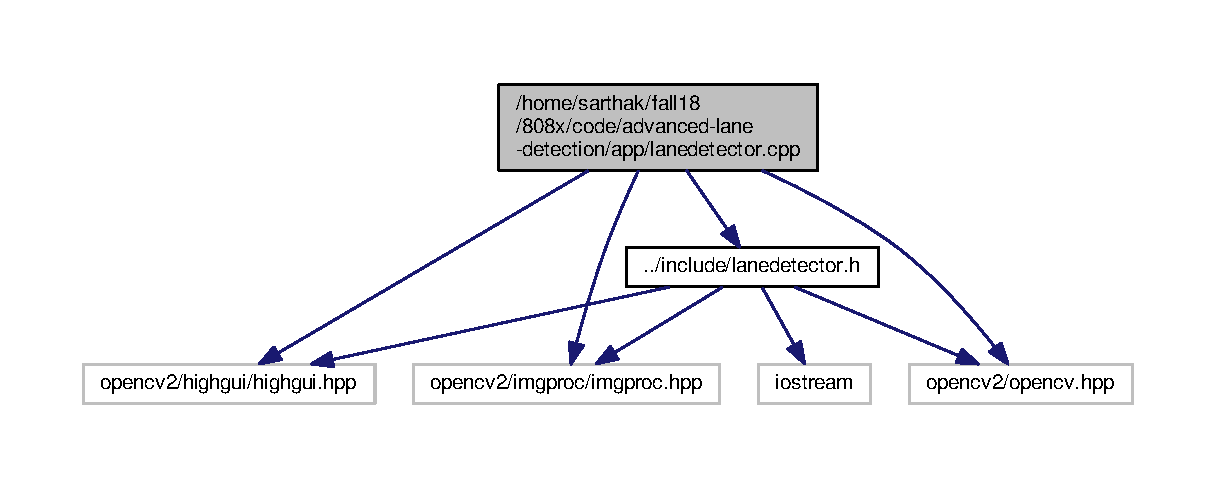
\includegraphics[width=350pt]{lanedetector_8cpp__incl}
\end{center}
\end{figure}


\subsection{Detailed Description}
All methods for class lanedetector are defined here. Primary objective of an object of this class is to detect lanes in a given frame and return a frame with an augmented lane overlay for better visualization. 

M\+IT License

Copyright (c) 2018 Sarthak Mahajan

Permission is hereby granted, free of charge, to any person obtaining a copy of this software and associated documentation files (the \char`\"{}\+Software\char`\"{}), to deal in the Software without restriction, including without limitation the rights to use, copy, modify, merge, publish, distribute, sublicense, and/or sell copies of the Software, and to permit persons to whom the Software is furnished to do so, subject to the following conditions\+:

The above copyright notice and this permission notice shall be included in all copies or substantial portions of the Software.

T\+HE S\+O\+F\+T\+W\+A\+RE IS P\+R\+O\+V\+I\+D\+ED \char`\"{}\+A\+S I\+S\char`\"{}, W\+I\+T\+H\+O\+UT W\+A\+R\+R\+A\+N\+TY OF A\+NY K\+I\+ND, E\+X\+P\+R\+E\+SS OR I\+M\+P\+L\+I\+ED, I\+N\+C\+L\+U\+D\+I\+NG B\+UT N\+OT L\+I\+M\+I\+T\+ED TO T\+HE W\+A\+R\+R\+A\+N\+T\+I\+ES OF M\+E\+R\+C\+H\+A\+N\+T\+A\+B\+I\+L\+I\+TY, F\+I\+T\+N\+E\+SS F\+OR A P\+A\+R\+T\+I\+C\+U\+L\+AR P\+U\+R\+P\+O\+SE A\+ND N\+O\+N\+I\+N\+F\+R\+I\+N\+G\+E\+M\+E\+NT. IN NO E\+V\+E\+NT S\+H\+A\+LL T\+HE A\+U\+T\+H\+O\+RS OR C\+O\+P\+Y\+R\+I\+G\+HT H\+O\+L\+D\+E\+RS BE L\+I\+A\+B\+LE F\+OR A\+NY C\+L\+A\+IM, D\+A\+M\+A\+G\+ES OR O\+T\+H\+ER L\+I\+A\+B\+I\+L\+I\+TY, W\+H\+E\+T\+H\+ER IN AN A\+C\+T\+I\+ON OF C\+O\+N\+T\+R\+A\+CT, T\+O\+RT OR O\+T\+H\+E\+R\+W\+I\+SE, A\+R\+I\+S\+I\+NG F\+R\+OM, O\+UT OF OR IN C\+O\+N\+N\+E\+C\+T\+I\+ON W\+I\+TH T\+HE S\+O\+F\+T\+W\+A\+RE OR T\+HE U\+SE OR O\+T\+H\+ER D\+E\+A\+L\+I\+N\+GS IN T\+HE S\+O\+F\+T\+W\+A\+RE. \begin{DoxyCopyright}{Copyright}
Copyright (c) 2018 Sarthak Mahajan
\end{DoxyCopyright}
\begin{DoxyAuthor}{Author}
Sarthak Mahajan 
\end{DoxyAuthor}

\hypertarget{lanedetector_8h}{}\section{/home/sarthak/fall18/808x/code/advanced-\/lane-\/detection/include/lanedetector.h File Reference}
\label{lanedetector_8h}\index{/home/sarthak/fall18/808x/code/advanced-\/lane-\/detection/include/lanedetector.\+h@{/home/sarthak/fall18/808x/code/advanced-\/lane-\/detection/include/lanedetector.\+h}}


Header file for the Lanedetector class.  


{\ttfamily \#include $<$iostream$>$}\\*
{\ttfamily \#include \char`\"{}opencv2/highgui/highgui.\+hpp\char`\"{}}\\*
{\ttfamily \#include \char`\"{}opencv2/imgproc/imgproc.\+hpp\char`\"{}}\\*
{\ttfamily \#include \char`\"{}opencv2/opencv.\+hpp\char`\"{}}\\*
Include dependency graph for lanedetector.\+h\+:
\nopagebreak
\begin{figure}[H]
\begin{center}
\leavevmode
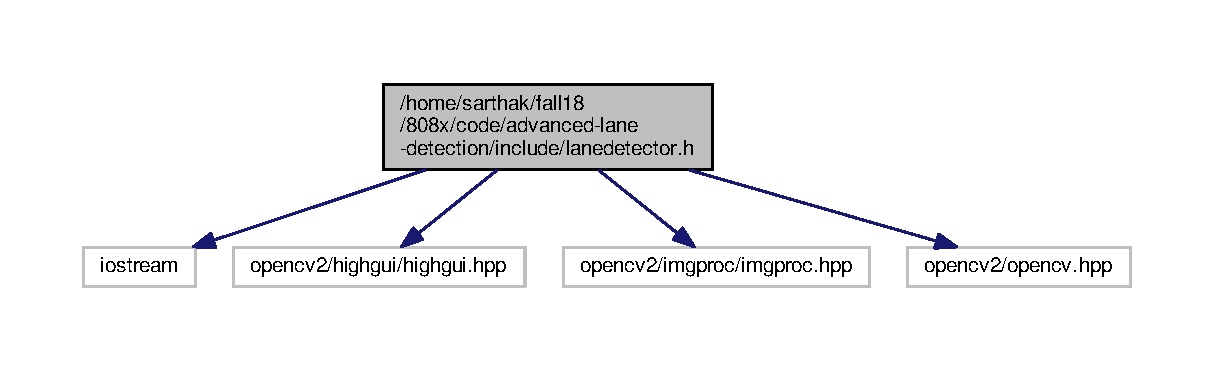
\includegraphics[width=350pt]{lanedetector_8h__incl}
\end{center}
\end{figure}
This graph shows which files directly or indirectly include this file\+:
\nopagebreak
\begin{figure}[H]
\begin{center}
\leavevmode
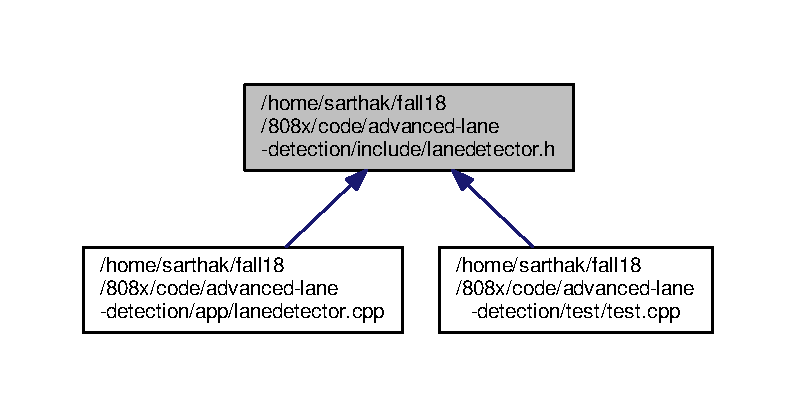
\includegraphics[width=350pt]{lanedetector_8h__dep__incl}
\end{center}
\end{figure}
\subsection*{Classes}
\begin{DoxyCompactItemize}
\item 
class \hyperlink{classlanedetector}{lanedetector}
\end{DoxyCompactItemize}


\subsection{Detailed Description}
Header file for the Lanedetector class. 

M\+IT License

Copyright (c) 2018 Sarthak Mahajan

Permission is hereby granted, free of charge, to any person obtaining a copy of this software and associated documentation files (the \char`\"{}\+Software\char`\"{}), to deal in the Software without restriction, including without limitation the rights to use, copy, modify, merge, publish, distribute, sublicense, and/or sell copies of the Software, and to permit persons to whom the Software is furnished to do so, subject to the following conditions\+:

The above copyright notice and this permission notice shall be included in all copies or substantial portions of the Software.

T\+HE S\+O\+F\+T\+W\+A\+RE IS P\+R\+O\+V\+I\+D\+ED \char`\"{}\+A\+S I\+S\char`\"{}, W\+I\+T\+H\+O\+UT W\+A\+R\+R\+A\+N\+TY OF A\+NY K\+I\+ND, E\+X\+P\+R\+E\+SS OR I\+M\+P\+L\+I\+ED, I\+N\+C\+L\+U\+D\+I\+NG B\+UT N\+OT L\+I\+M\+I\+T\+ED TO T\+HE W\+A\+R\+R\+A\+N\+T\+I\+ES OF M\+E\+R\+C\+H\+A\+N\+T\+A\+B\+I\+L\+I\+TY, F\+I\+T\+N\+E\+SS F\+OR A P\+A\+R\+T\+I\+C\+U\+L\+AR P\+U\+R\+P\+O\+SE A\+ND N\+O\+N\+I\+N\+F\+R\+I\+N\+G\+E\+M\+E\+NT. IN NO E\+V\+E\+NT S\+H\+A\+LL T\+HE A\+U\+T\+H\+O\+RS OR C\+O\+P\+Y\+R\+I\+G\+HT H\+O\+L\+D\+E\+RS BE L\+I\+A\+B\+LE F\+OR A\+NY C\+L\+A\+IM, D\+A\+M\+A\+G\+ES OR O\+T\+H\+ER L\+I\+A\+B\+I\+L\+I\+TY, W\+H\+E\+T\+H\+ER IN AN A\+C\+T\+I\+ON OF C\+O\+N\+T\+R\+A\+CT, T\+O\+RT OR O\+T\+H\+E\+R\+W\+I\+SE, A\+R\+I\+S\+I\+NG F\+R\+OM, O\+UT OF OR IN C\+O\+N\+N\+E\+C\+T\+I\+ON W\+I\+TH T\+HE S\+O\+F\+T\+W\+A\+RE OR T\+HE U\+SE OR O\+T\+H\+ER D\+E\+A\+L\+I\+N\+GS IN T\+HE S\+O\+F\+T\+W\+A\+RE. \begin{DoxyCopyright}{Copyright}
Copyright (c) 2018 Sarthak Mahajan
\end{DoxyCopyright}
\begin{DoxyAuthor}{Author}
Sarthak Mahajan All methods and variables have been declared here and defined in \hyperlink{lanedetector_8cpp}{lanedetector.\+cpp} 
\end{DoxyAuthor}

\hypertarget{test_8cpp}{}\section{/home/sarthak/fall18/808x/code/advanced-\/lane-\/detection/test/test.cpp File Reference}
\label{test_8cpp}\index{/home/sarthak/fall18/808x/code/advanced-\/lane-\/detection/test/test.\+cpp@{/home/sarthak/fall18/808x/code/advanced-\/lane-\/detection/test/test.\+cpp}}


All tests are defined here. Primarily to check image channels and predicted turns.  


{\ttfamily \#include $<$iostream$>$}\\*
{\ttfamily \#include $<$gtest/gtest.\+h$>$}\\*
{\ttfamily \#include \char`\"{}opencv2/highgui/highgui.\+hpp\char`\"{}}\\*
{\ttfamily \#include \char`\"{}opencv2/imgproc/imgproc.\+hpp\char`\"{}}\\*
{\ttfamily \#include \char`\"{}opencv2/opencv.\+hpp\char`\"{}}\\*
{\ttfamily \#include \char`\"{}../include/lanedetector.\+hpp\char`\"{}}\\*
Include dependency graph for test.\+cpp\+:
\nopagebreak
\begin{figure}[H]
\begin{center}
\leavevmode
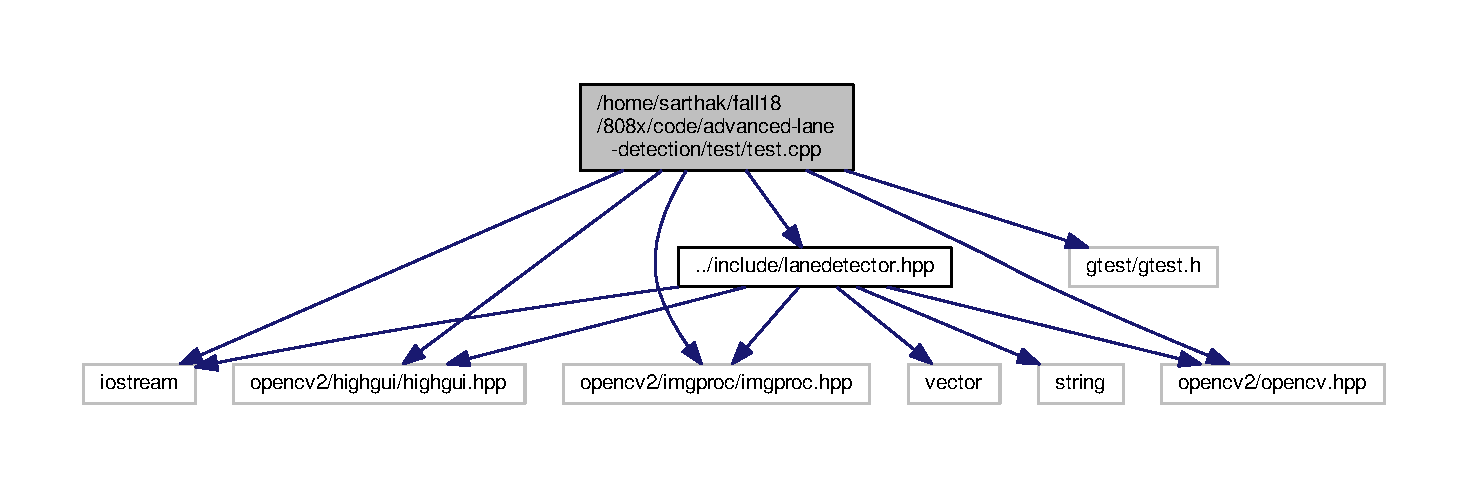
\includegraphics[width=350pt]{test_8cpp__incl}
\end{center}
\end{figure}
\subsection*{Functions}
\begin{DoxyCompactItemize}
\item 
{\bfseries T\+E\+ST} (channels, test\+Num\+Of\+Channels\+Returned)\hypertarget{test_8cpp_ad32156f46a4683e5bc125eb215ae5931}{}\label{test_8cpp_ad32156f46a4683e5bc125eb215ae5931}

\item 
{\bfseries T\+E\+ST} (turns, check\+Turn\+Direction\+Left)\hypertarget{test_8cpp_a0640a377302f116dfb1fd51f2b9584bb}{}\label{test_8cpp_a0640a377302f116dfb1fd51f2b9584bb}

\item 
{\bfseries T\+E\+ST} (turns, check\+Turn\+Direction\+Right)\hypertarget{test_8cpp_a710b6f5f19458db23dbd7233e241b467}{}\label{test_8cpp_a710b6f5f19458db23dbd7233e241b467}

\end{DoxyCompactItemize}


\subsection{Detailed Description}
All tests are defined here. Primarily to check image channels and predicted turns. 

M\+IT License

Copyright (c) 2018 Sarthak Mahajan

Permission is hereby granted, free of charge, to any person obtaining a copy of this software and associated documentation files (the \char`\"{}\+Software\char`\"{}), to deal in the Software without restriction, including without limitation the rights to use, copy, modify, merge, publish, distribute, sublicense, and/or sell copies of the Software, and to permit persons to whom the Software is furnished to do so, subject to the following conditions\+:

The above copyright notice and this permission notice shall be included in all copies or substantial portions of the Software.

T\+HE S\+O\+F\+T\+W\+A\+RE IS P\+R\+O\+V\+I\+D\+ED \char`\"{}\+A\+S I\+S\char`\"{}, W\+I\+T\+H\+O\+UT W\+A\+R\+R\+A\+N\+TY OF A\+NY K\+I\+ND, E\+X\+P\+R\+E\+SS OR I\+M\+P\+L\+I\+ED, I\+N\+C\+L\+U\+D\+I\+NG B\+UT N\+OT L\+I\+M\+I\+T\+ED TO T\+HE W\+A\+R\+R\+A\+N\+T\+I\+ES OF M\+E\+R\+C\+H\+A\+N\+T\+A\+B\+I\+L\+I\+TY, F\+I\+T\+N\+E\+SS F\+OR A P\+A\+R\+T\+I\+C\+U\+L\+AR P\+U\+R\+P\+O\+SE A\+ND N\+O\+N\+I\+N\+F\+R\+I\+N\+G\+E\+M\+E\+NT. IN NO E\+V\+E\+NT S\+H\+A\+LL T\+HE A\+U\+T\+H\+O\+RS OR C\+O\+P\+Y\+R\+I\+G\+HT H\+O\+L\+D\+E\+RS BE L\+I\+A\+B\+LE F\+OR A\+NY C\+L\+A\+IM, D\+A\+M\+A\+G\+ES OR O\+T\+H\+ER L\+I\+A\+B\+I\+L\+I\+TY, W\+H\+E\+T\+H\+ER IN AN A\+C\+T\+I\+ON OF C\+O\+N\+T\+R\+A\+CT, T\+O\+RT OR O\+T\+H\+E\+R\+W\+I\+SE, A\+R\+I\+S\+I\+NG F\+R\+OM, O\+UT OF OR IN C\+O\+N\+N\+E\+C\+T\+I\+ON W\+I\+TH T\+HE S\+O\+F\+T\+W\+A\+RE OR T\+HE U\+SE OR O\+T\+H\+ER D\+E\+A\+L\+I\+N\+GS IN T\+HE S\+O\+F\+T\+W\+A\+RE. \begin{DoxyCopyright}{Copyright}
Copyright (c) 2018 Sarthak Mahajan
\end{DoxyCopyright}
\begin{DoxyAuthor}{Author}
Sarthak Mahajan 
\end{DoxyAuthor}

%--- End generated contents ---

% Index
\backmatter
\newpage
\phantomsection
\clearemptydoublepage
\addcontentsline{toc}{chapter}{Index}
\printindex

\end{document}
